\section{Data Journalist Agent}
\label{sec:method}

Given any raw data $\mathcal{D}$, the goal of \method\ is to produce an article $\mathcal{U}$ that is narratively compelling, visually appealing, and verifiable in its content.
\begin{figure*}[!t]
    \centering
    
\includegraphics[width=\textwidth]{fig/pipeline.pdf}
    \caption{\textbf{The Virtual Newsroom for \methodshort{}.} A raw dataset $\mathcal{D}$ flows through a sequence of specialist roles: the \textit{Detective} gathers external context $\widetilde{\mathcal{D}}$ from the web, the \textit{Analyst} writes Python code $\mathcal{C}$ and emits results $\mathcal{R}$ with code-line provenance $\mathcal{R} \xleftarrow{\mathcal{C}} \mathcal{D} \cup \widetilde{\mathcal{D}}$, the \textit{Editor} drafts several findings $\mathcal{F}$ from different angles, the \textit{Designer} produces multimedia assets $\mathcal{V}$ via tool calls, and the \textit{Programmer} renders the final HTML $\mathcal{U}$. The page is then audited by the \textit{Auditor}, which provides suggestions $\mathcal{S}$ for visual and structural defects, and the \textit{Inspector}, which binds every published claim back to its supporting evidence $\mathcal{E} = {\mathcal{D}} \cup \mathcal{R} \cup \mathcal{C} \cup \mathcal{F} \cup \mathcal{V}$. Each role produces a set of intermediate elements (grey); those that ground the final article are highlighted (red outline), and the Inspector links them into a traceable evidence chain.}
    \label{fig:pipeline}
\vspace{-1em}
\end{figure*}

\subsection{The Virtual Newsroom}
\label{sec:method:roles}

As illustrated in Figure \ref{fig:pipeline}, we define our multi-agent solution as a virtual newsroom composed of specialised agent roles.

\paragraph{Detective.}
A raw data source is rarely enough on its own: an article almost always depends on context the dataset does not contain. For example, historical events often need to be associated with the time the data were released. The Detective gathers this context before any number is computed, so that downstream roles can frame the data rather than invent claims about it. Concretely, it augments the raw dataset $\mathcal{D}$ via web search into an enriched corpus $\mathcal{D} \cup \widetilde{\mathcal{D}}$, where $\widetilde{\mathcal{D}} \xleftarrow{\text{Web search}} \mathcal{D}$ contains additional context items tagged with category and source URLs, together with a small library of reference media (photographs, maps, short clips) that other agents can later reuse.

\paragraph{Analyst.}
A news article typically cites dozens of statistics to arrive at its insights. However, given a dataset, it is rarely clear in advance which statistical findings it admits, or which of them will prove most meaningful. The Analyst therefore prioritises completeness: it enumerates every analysis the dataset can support, profiles every column, and runs actual code rather than asking the model to estimate. From the augmented dataset, it derives a set of results $\mathcal{R}=\{r_i\}$ and supporting code $\mathcal{C}=\{c_i\}$ with $r_i \xleftarrow{c_i} \mathcal{D} \cup \widetilde{\mathcal{D}}$, where each finding $r_i$ carries a pointer to the script $c_i$ that generated it,  ensuring that every outcome is traceable.

\paragraph{Editor.}
An interesting analysis is not yet a story. Given a set of findings, the Editor decides what the article actually argues: which findings should lead, which should support, which add colour, and which should be cut. Reasoning over the Analyst's findings, it produces an editorial plan $\mathcal{F} \xleftarrow{\text{LLM}} \mathcal{R}$ that ranks each item by priority, selects the items worth keeping, and drafts a paragraph-level prose outline. Each finding $f_i$ in $\mathcal{F}$ is annotated with the upstream items it draws on, $f_i \sim (r_i, c_i)$.

\paragraph{Designer.}
An article is not just plain text: multimedia elements can substantially improve readability, such as maps for geography, audio for music, video for events, and interactive widgets for complex findings. For each finding $f_i$ of the editorial plan, the Designer reasons about what a reader would most want to see, then selects the medium that best fits the data, drawing on a suite of external generative tools such as text-to-image and text-to-video. The resulting per-section visual assets $\mathcal{V} \xleftarrow{\text{Tool}} \mathcal{F}$ include the corresponding asset calls needed to realise each medium, where we store every prompt or parameter.

\paragraph{Programmer.}
Static formats such as PDF cannot natively coordinate multimedia elements; an HTML webpage, by contrast, is the ideal medium for what a reader actually sees. We therefore introduce a Programmer that renders the final page in HTML from the upstream artifacts. The Programmer generates no new facts or numbers; it operates in two modes. (i) In assembly mode, it quotes the upstream artifacts $\{\mathcal{F}, \mathcal{V}\}$ and composes them into a complete interactive article $\mathcal{U} \xleftarrow{} \{\mathcal{F}, \mathcal{V}\}$. (ii) In revision mode, it additionally takes the Auditor's revision suggestions $\mathcal{S}$ and revises the page accordingly, forwarding the audited article $\mathcal{U} \xleftarrow{} \{\mathcal{U}, \mathcal{S}\}$ to the Inspector.

\paragraph{Auditor.}
The rendered HTML may still harbour visual or structural defects: overlapping elements, broken charts, missing assets, or unresponsive interactions. Such defects can quietly undermine an otherwise well-grounded story. The Auditor therefore reviews the rendered page, $\mathcal{S} \xleftarrow{} \mathcal{U}$, and flags these issues; it returns the page to the Programmer for repair.

\subsection{How to ensure claims are verifiable?}
\label{sec:method:trace}

\begin{figure}[!h]
\centering
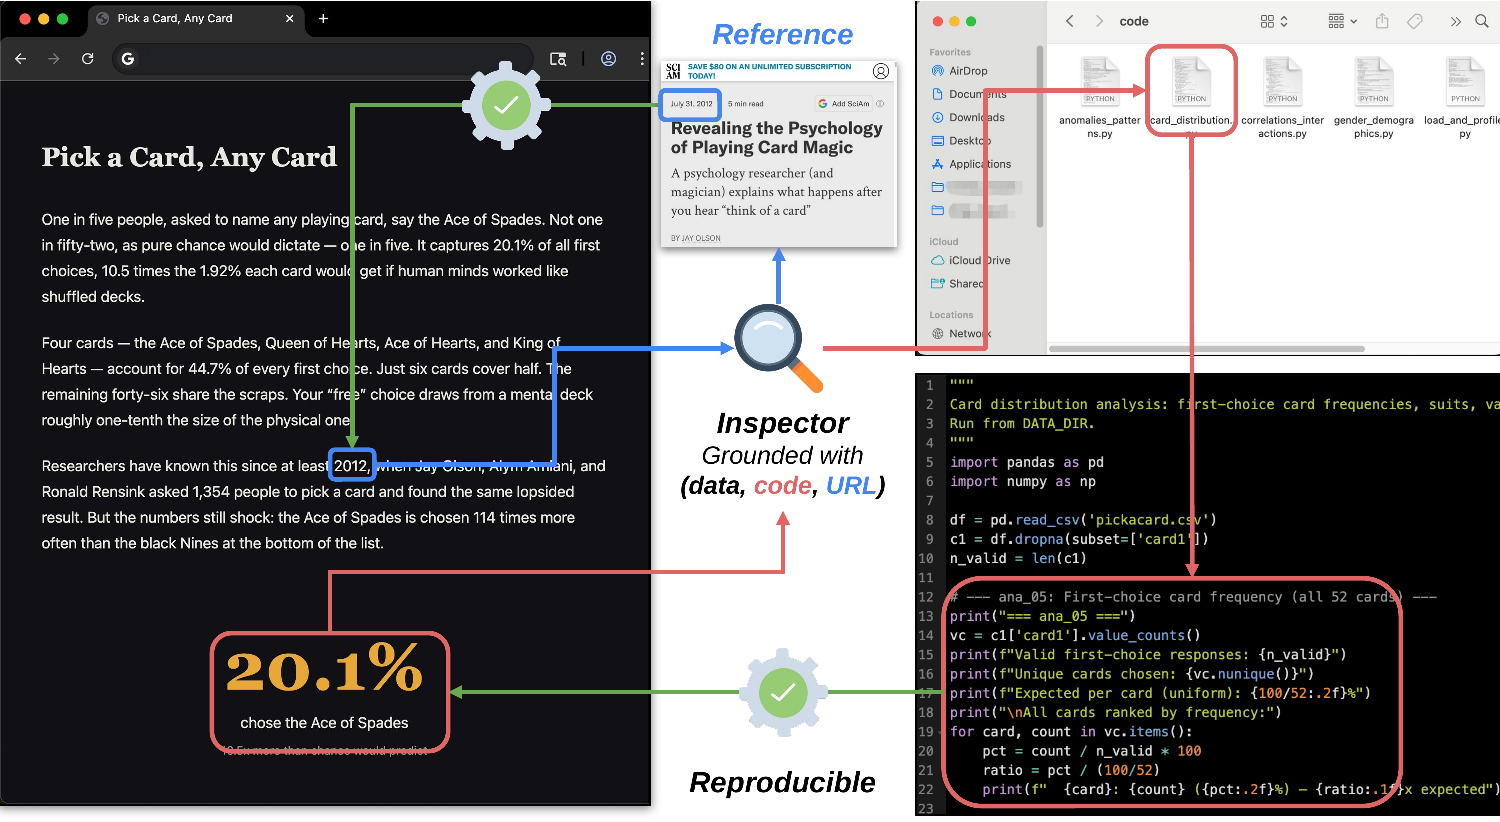
\includegraphics[width=\linewidth]{fig/evidence.pdf}
\caption{\textbf{Illustration of the Inspector.} The Inspector binds every output finding back to its supporting evidence, which falls into two types: (i) \textit{code evidence}, the source file and specific line that produced a reported number, and (ii) \textit{reference evidence}, the external article or URL that grounds a contextual claim. The binding establishes auditability / traceability rather than factual correctness.
}
\vspace{-1em}
\label{fig:viewer}
\end{figure}


\paragraph{Inspector \faSearch.}
A central challenge for any multi-agent system that produces an article is that the reader has no reason to trust the page unless every visible element, from the lede sentence to the final tooltip, resolves to something concrete upstream (such as code or reference). We therefore introduce the Inspector, which closes this loop at the level of individual items.

We let all upstream agents each contribute \textit{atomic units of evidence}. 
The Detective contributes a context ${\mathcal{D}} = \{d_i\}$, where each $d_i$ is a context item with a source URL. The Analyst contributes findings $\mathcal{R} = \{r_j\}$ paired one-to-one with code $\mathcal{C} = \{c_j\}$, so that every $r_j$ is supported by the script $c_j$ that produced it. The Editor contributes a finding $\mathcal{F} = \{f_k\}$, where each $f_k$ is a paragraph with upstream pointers, and the Designer contributes specifications $\mathcal{V} = \{v_\ell\}$, where each $v_\ell$ is a per-section specification, and we record the tool call and parameters (such as prompts).
Together these form the pool of upstream evidence $\mathcal{E} = {\mathcal{D}} \cup \mathcal{R} \cup \mathcal{C} \cup \mathcal{F} \cup \mathcal{V}$.

The Inspector decomposes the audited page into a set of partial findings $\mathcal{U} = \{u_m\}$, where each $u_m$ is a self-contained HTML fragment realising a sentence, chart, or interactive element. It then binds every fragment $u_m$ to the entries of the evidence base $\mathcal{E}$ that ground it, \ie~$u_m \sim (d_i, r_j, c_j, f_k, v_l)$, so that each fragment carries an explicit link back to the evidence from which it was derived. 

The Inspector recognises two types of evidence link, as illustrated in Figure~\ref{fig:viewer}: \textit{code evidence}, where a claim traces back to the specific script and line that produced it, and \textit{reference evidence}, where a contextual claim is grounded in an external URL. 
The result is a page where truthfulness is \textbf{evidence-traceable}: every claim can be followed back through the Programmer, the Designer, and the Analyst to the original data file or source reference.